\section{Results and Discussion}
\label{sec:results}
We first provide the results of the case study. Then we give more general results about the application of conflict-measuring methods to multiple multi-objective systems.

\subsection{Case Study Results}
We parameterized and solved the multi-objective model (\eqref{eqn:objFire}-\eqref{eqn:constraintNonNeg}) for each of the climate scenarios, generating three efficient frontiers: $Z_{\text{None}}$, $Z_{E45}$, and $Z_{E85}$ for the None, Ensemble RCP 4.5, and Ensemble RCP 8.5 scenarios, respectively. The frontiers are shown in Figure \ref{fig:frontiersAll}; their summary details are shown in Table \ref{tab:frontiersSummary}.

\begin{table}[]
\centering
\caption[Summary of efficient frontiers]{Summary of the performance of the efficient frontiers for each climate change scenario.}
\label{tab:frontiersSummary}
\begin{tabular}{lllll}
\multicolumn{2}{l|}{}                                                  & \textbf{None} & \textbf{E45} & \textbf{E85} \\ \hline
\multicolumn{2}{l|}{\textbf{Hypervolume}}                              & 0.876977      & 0.866857     & 0.829541     \\ \hline
\multirow{3}{*}{\textbf{Fire hazard}}       & \multicolumn{1}{l|}{min} & 21321.21      & 23219.82     & 23268.02     \\
                                            & \multicolumn{1}{l|}{max} & 21933.29      & 23973.79     & 23724.98     \\
                                            & \multicolumn{1}{l|}{avg} & 21406.26      & 23324.41     & 23369.57     \\ \hline
\multirow{3}{*}{\textbf{NSO habitat}}       & \multicolumn{1}{l|}{min} & 2532.33       & 2412.18      & 2171.10      \\
                                            & \multicolumn{1}{l|}{max} & 2540.05       & 2477.18      & 2481.01      \\
                                            & \multicolumn{1}{l|}{avg} & 2536.31       & 2447.92      & 2421.99      \\ \hline
\multirow{3}{*}{\textbf{Sediment delivery}} & \multicolumn{1}{l|}{min} & 0             & 0            & 0            \\
                                            & \multicolumn{1}{l|}{max} & 24.57         & 63.43        & 69.68        \\
                                            & \multicolumn{1}{l|}{avg} & 10.25         & 27.98        & 31.19        \\ \hline
\multicolumn{2}{l}{\textbf{Number of solutions}}                       & 51            & 701          & 1083        
\end{tabular}
\end{table}


\begin{figure}[ht!]
  \subfloat[None]{%
    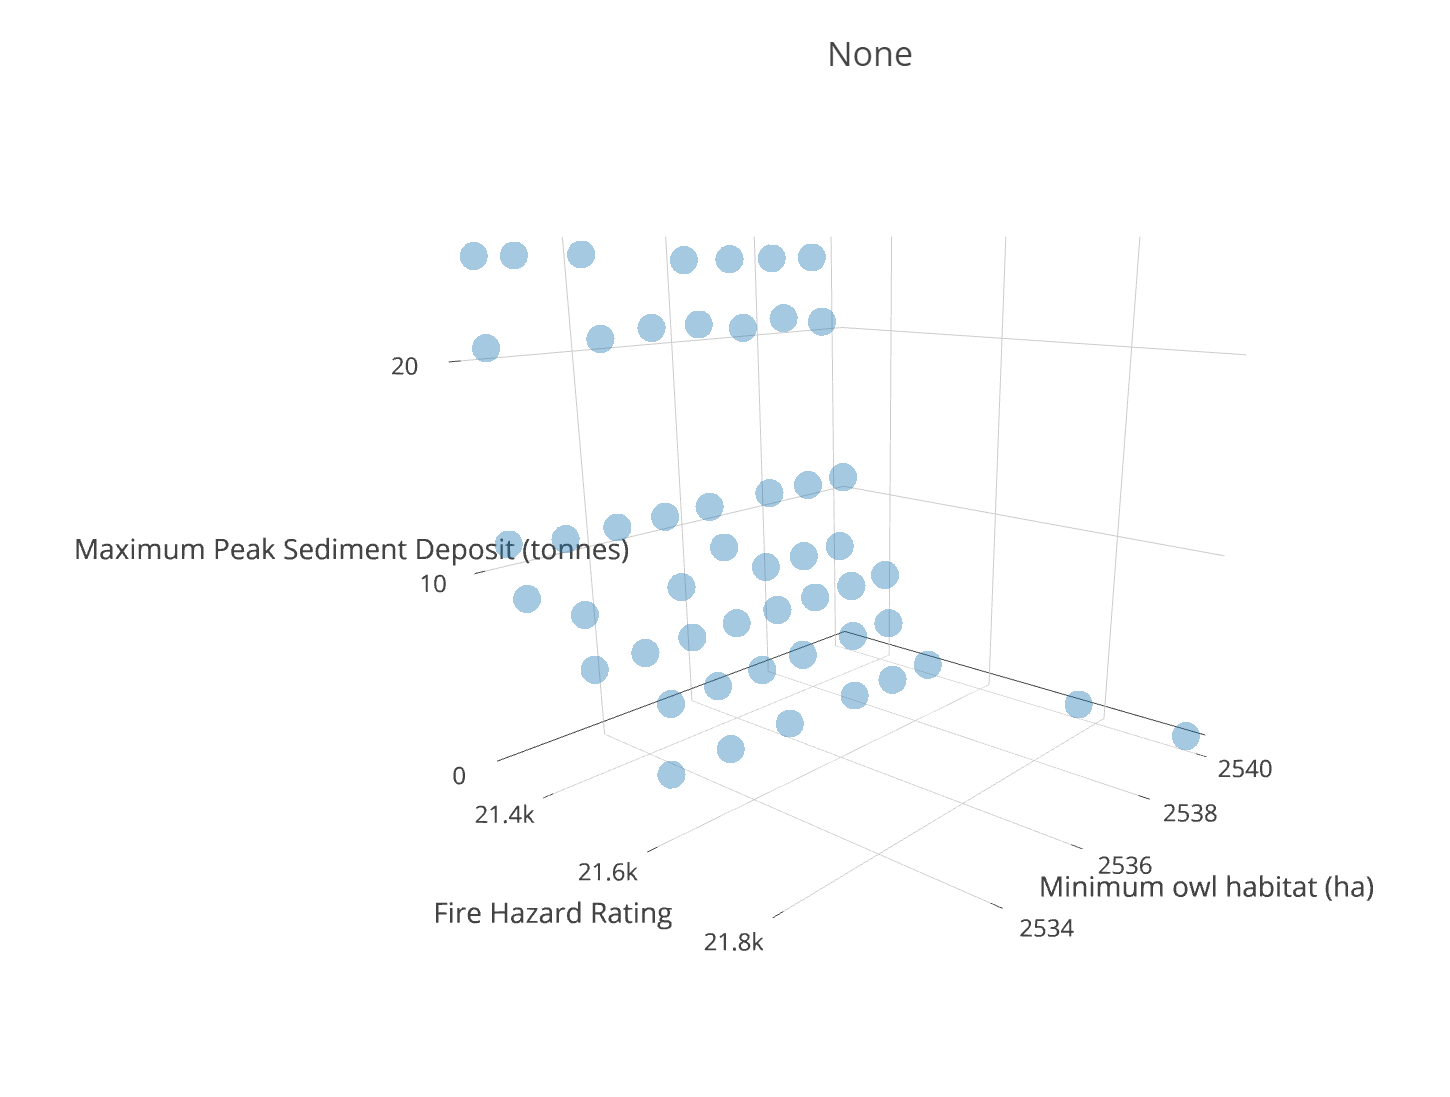
\includegraphics[width=.45\textwidth]{../images/Frontier_None}%
    \label{fig:frontierNone}%
  }
  \subfloat[Ensemble RCP 4.5]{%
    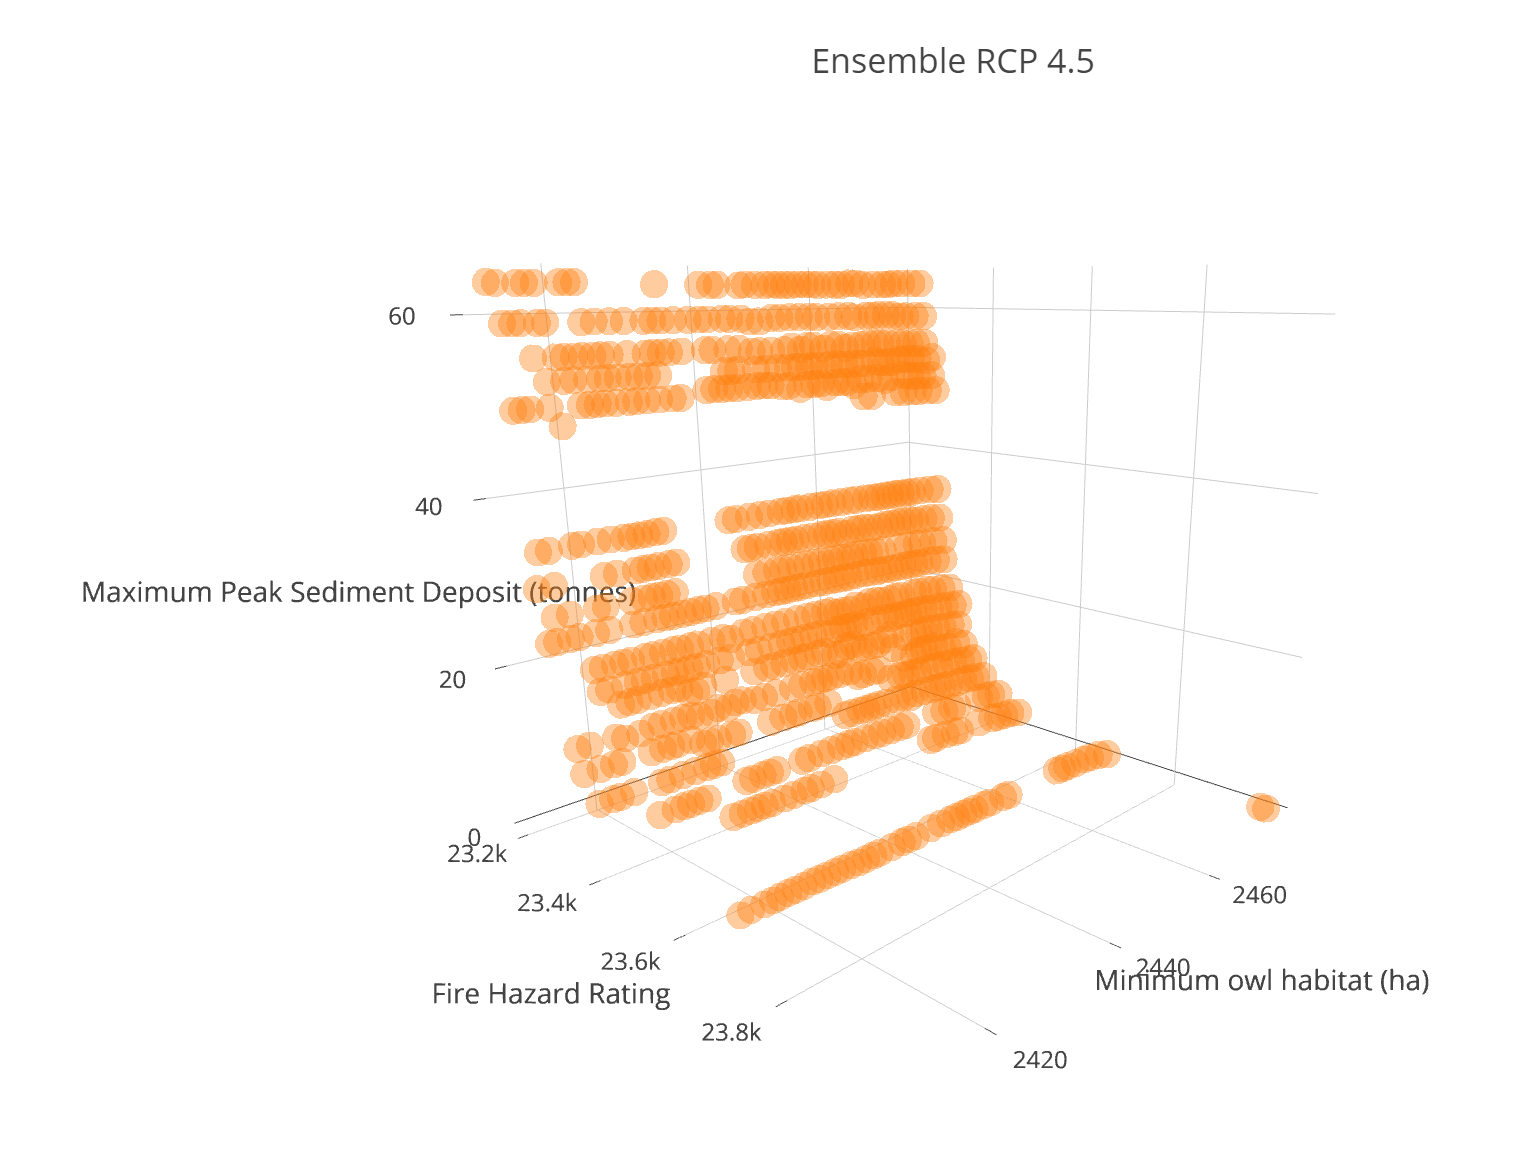
\includegraphics[width=.45\textwidth]{../images/Frontier_E45}%
    \label{fig:frontierE45}%
  }\hfill\centering
  \subfloat[Ensemble RCP 8.5]{%
    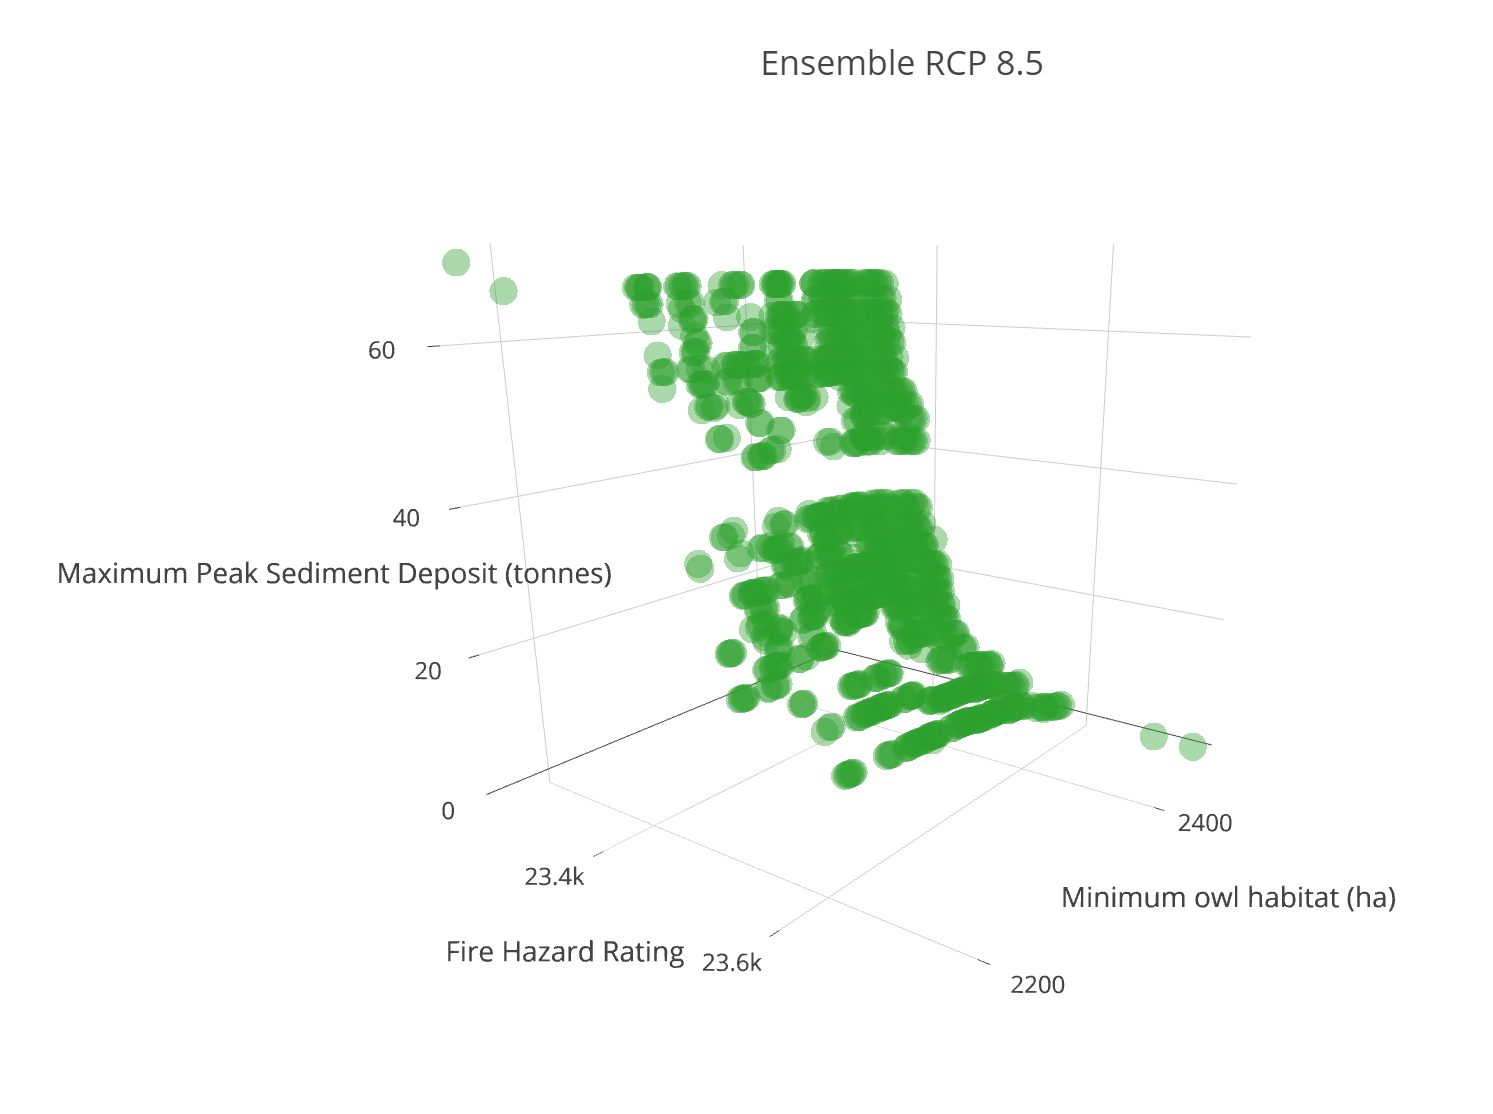
\includegraphics[width=.45\textwidth]{../images/Frontier_E85}%
    \label{fig:frontierE85}%
  }
  \caption[Frontiers for each climate change scenario]{Efficient frontiers for each climate change scenario.}
  \label{fig:frontiersAll}
\end{figure}

We begin our analysis by investigating the impacts of climate change on the provision of individual ecosystem services. We then consider how climate change impacts the joint provision of ecosystem services and the conflict among them.

\subsubsection{Individual ecosystem service achievement}
The average achievement of all ecosystem services decreases with increasing severity of climate change (see Table \ref{tab:frontiersSummary}, ``avg'' rows). We find the difference in ecosystem service provision greater between the assumption of no climate change and mild climate change (None to E45) than it is between mild climate change and severe climate change (E45 to E85). This suggests that, for the ecosystem services in this study, the realization of climate change is more significant than the severity of that change.

The model data provide evidence of why this is the case. Consider Figure \ref{fig:avgSedimentDelivery}. This figure shows the average number of tonnes of sediment delivered as a result of performing fuel removals for each climate change scenario. The sediment delivery under E45 is nearly twice the sediment delivery under the None scenario (81\% higher), whereas the E85 scenario is only 0.4\% higher than the E45 scenario.

\begin{figure}[ht]
\centering
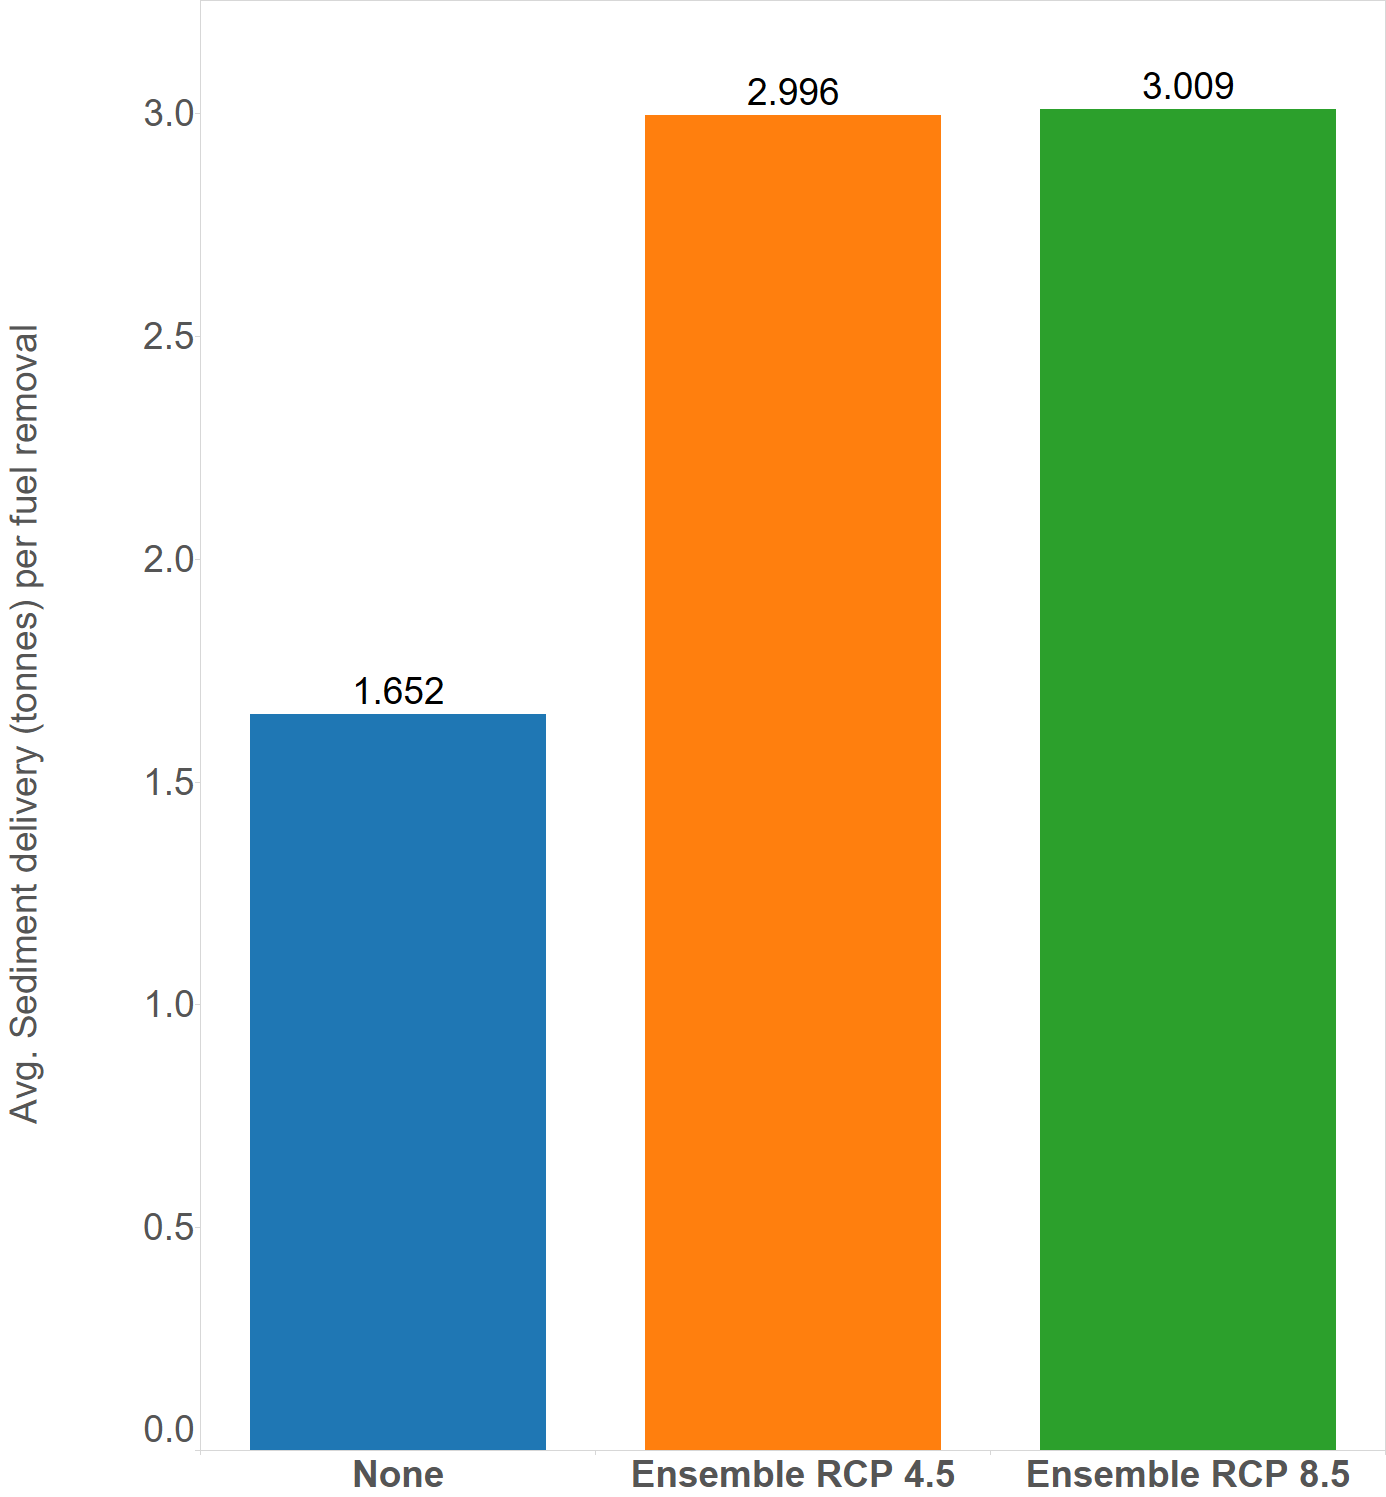
\includegraphics[width=.55\textwidth]{../images/AvgSedimentSpikes}
\caption[Average sediment delivery across climate scenarios]{Average spike in sediment delivery as a result of performing fuel removals for each of the climate change scenarios.}
\label{fig:avgSedimentDelivery}
\end{figure}

Similarly, see Figure \ref{fig:cumSmallestFireHazard}. The figure shows for each climate scenario, the resulting fire hazard for the Drink Area if the most successful fire hazard reduction techniques were performed. These numbers represent an unconstrained lower bound for the minimum fire hazard. We again notice a larger difference between None and E45 than between E45 and E85.

\begin{figure}[ht]
\centering
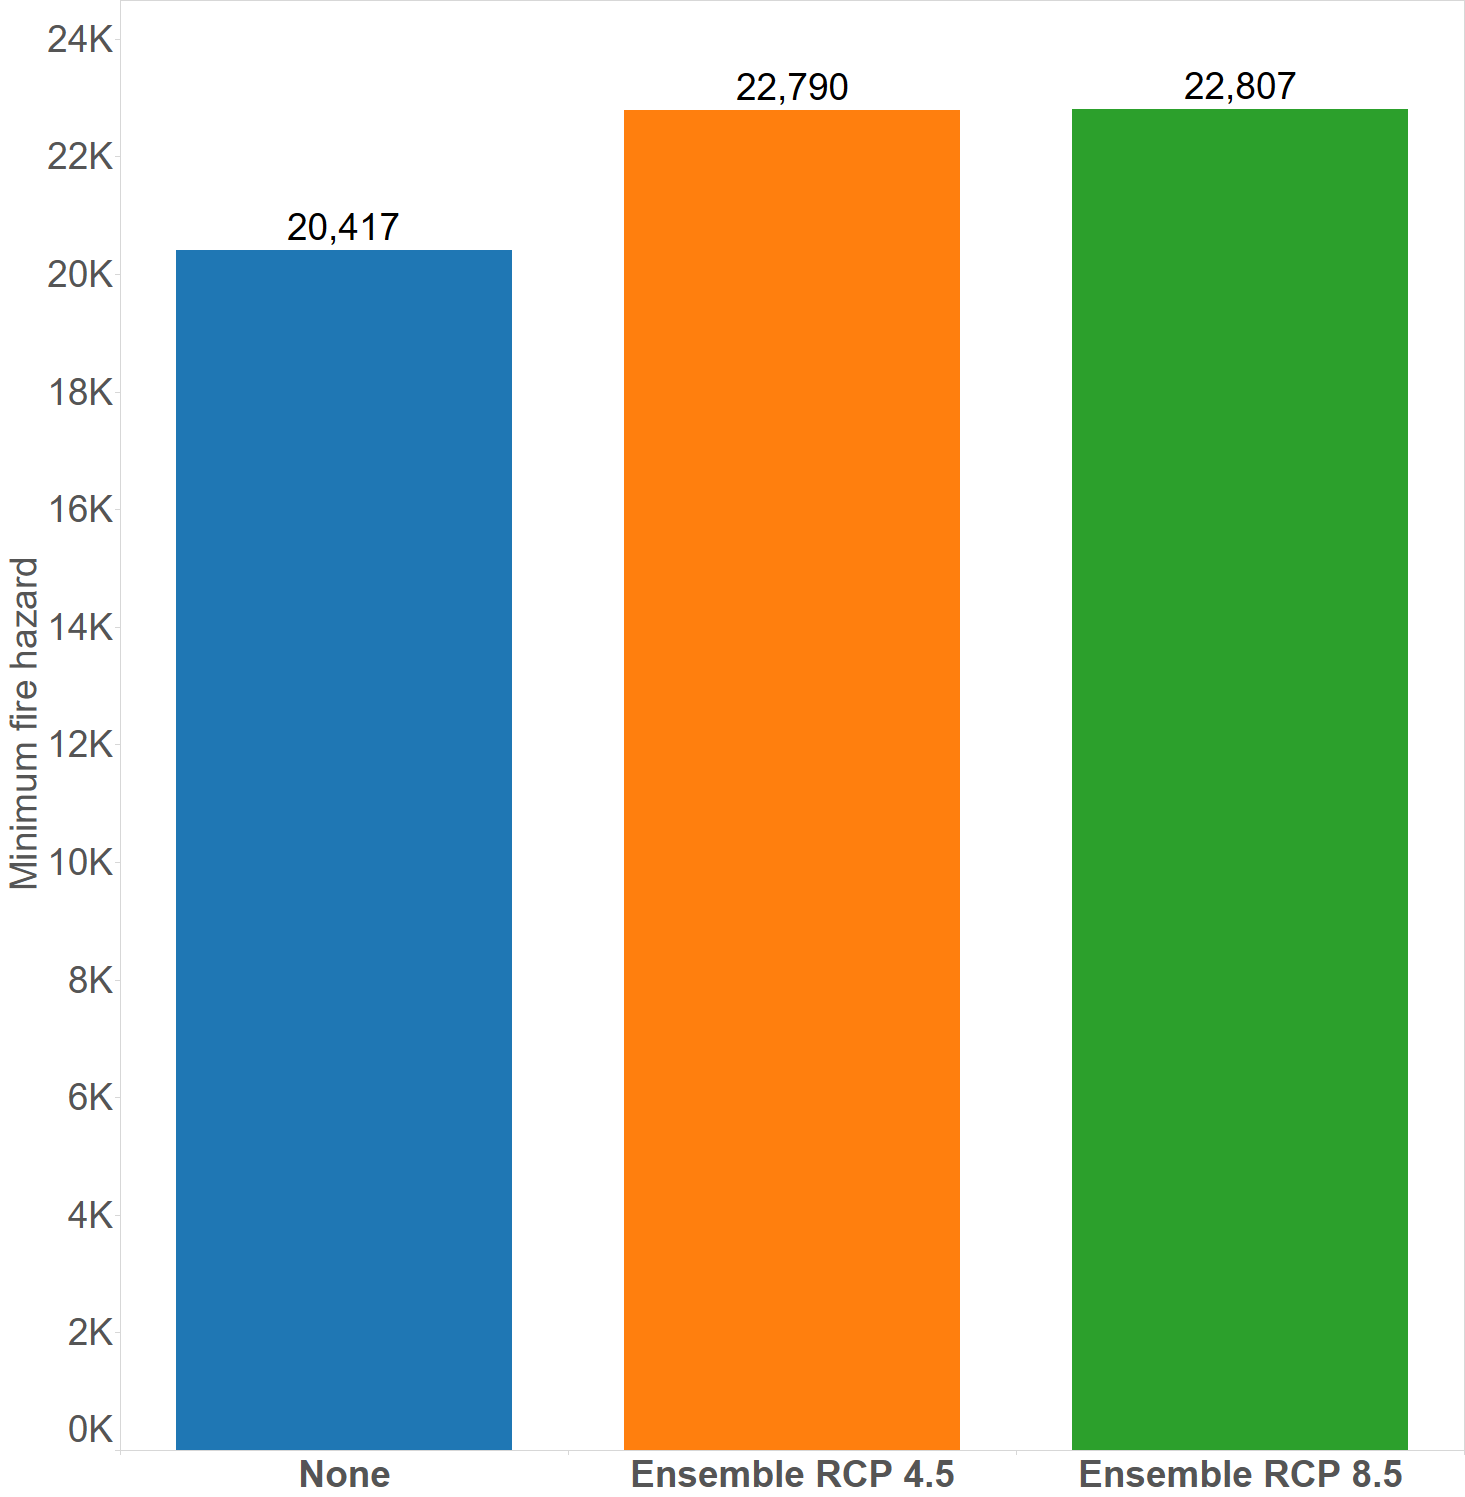
\includegraphics[width=.55\textwidth]{../images/CumSmallestFireHazard}
\caption[Lower bound on fire hazard for each climate scenario]{Shown here are lower bounds on the minimum fire hazard for the Drink Area under each climate change scenario. They represent the cumulative fire hazard if all constraints on fuel removals were ignored (inequalities \eqref{eqn:constraintAreaRestr}-\eqref{eqn:constraintAreaFlucU}).}
\label{fig:cumSmallestFireHazard}
\end{figure}

% Talk about sources of conflict in between objectives. Well, the conflict metric is higher for this frontier than for this frontier (graph of cross section). The underlying reason for this is bc the ?sed contrib is higher in this scenario than that scenario? or ?the efficacy of treatments is highest in E85 and on the stands located in the watershed?. Something like that. Look into treatment efficacy on WS stands across the climate scenarios. And the sediment contributions vs climate scenarios.

% Per stand, avg reduction in fire hazard vs sediment delivered as a result of fuel removal (same thing for reduc in fire hazard vs triggering NSO habitat)

% For a given fuel removal that disqualifies a stand as NSO habitat, what is the difference in fire hazard between the "NONE" and (whatever that fuel removal action was) is?